\section{Desarrollo de la librería}

La librería es nombrada como \textbf{L.A.M.F.R.I.A} que significa: Librería para el análisis de multifractalidad y robustez con algoritmos de inteligencia artificial.

\subsection{Procesamiento de redes con SNAP}

Este trabajo es desarrollado con el apoyo de la librería SNAP de la Universidad de Standford \url{https://snap.stanford.edu}, la cual está escrita en C++ y se encuentra optimizada para redes de gran tamaño, gracias al uso de una representación basada en matrices dispersas.

Para la implementación de los algoritmos se utiliza el lenguaje de Programación Python y el entorno que ofrece esta librería para este lenguaje. La elección del lenguaje se debe a que actualmente es tendencia para el desarrollo de aplicaciones Inteligencia Artificial, el cual es el enfoque de este proyecto. Esto permite a futuro los algoritmos utilizados puedan ser integradas con mayor facilidad con otras estrategias de inteligencia artificial.

\subsubsection{¿Porque SNAP?}

En el mercado se destacan algunas librerías para el procesamiento de redes complejas como:

\begin{itemize}
    \item NetworkX: Es una librería de Python comúnmente utilizadas, pero no es recomendada con redes de más de 100000 nodos
    \item IGraph: Utilizada en Python y R, está enfocada a estudio de propiedades y representación gráfica que a procesamiento de redes de gran tamaño.
    \item sigma.js, escrita en JavaScript, sin embargo, el lenguaje no es recomendado para procesamiento si no para visualización.
\end{itemize}


\subsection{Arquitectura de la librería}

La librería desarrollada es un conjunto de funciones que corren sobre SNAP. En la figura \ref{fig:diagramaConceptual} se provee un diagrama conceptual de la librería.

\begin{figure}[H]
    \centering
    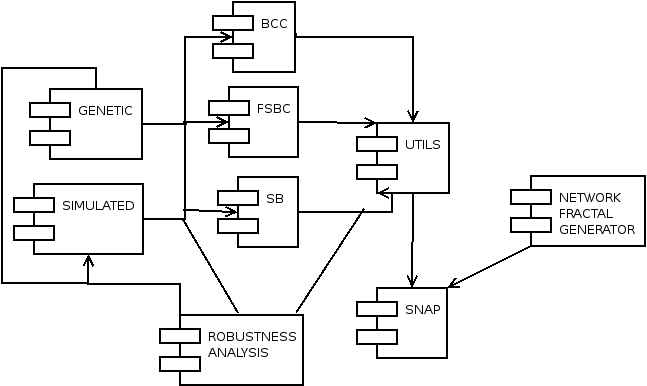
\includegraphics[scale=0.7]{Capitulo7Libreria/imagenes/componentes.png}
    \caption{Diagrama conceptual de L.A.M.F.R.I.A}
    \label{fig:diagramaConceptual}
\end{figure}

\begin{itemize}
    \item SNAP: Provee las funciones de carga y búsqeuda en redes complejas
    \item UTILS: Provee funciones generales para los algoritmos, como es el caso de calculo de matrices de adyacencia o conectividad. Así mismo funciones para la carga y guardado de archivos
    \item BCC: Algoritmo de Box Compact Counting
    \item FSBC: Algoritmo de Fixed Size Box Counting
    \item DB: Algoritmo de SandBox
    \item Network Fractal Generator: Ofrece funciones para la creación de (2,2)-flower y (1,3)-flower de cualquier generación
    \item Genetic y Simulated ofrecen las estrategias de IA. Estas hacen parte de la ejecución de los algoritmos ya que calculan los centros de cajas y se ejecuta el algoritmo con esta configuración
    \item Robustness Analysis: Realiza el análisis de robustez, permite utiliza todos los algoritmos para el análisis de multifractalidad a medida que se pierden nodos. En las pruebas solo se usó el algoritmo SandBox por cuestiones de tiempo.
\end{itemize}